%%%%% Don't Make Changes Below Here %%%%%
\documentclass{article}\usepackage[utf8]{inputenc}\usepackage[margin=0.4cm,top=0.4cm,bottom=0.4cm]{geometry}\usepackage[usenames,dvipsnames,svgnames,table]{xcolor}
\usepackage{calligra}\usepackage{tikz}\usepackage{hyperref}\usetikzlibrary{matrix,fit,chains,calc,scopes}\usepackage{tcolorbox}\tcbuselibrary{skins}\tcbset{Baystyle/.style={sharp corners,enhanced,boxrule=6pt,colframe=orange,height=\textheight,width=\textwidth,borderline={8pt}{-11pt}{},}}\usepackage{amsmath,amssymb,amsthm,tikz,tkz-graph,color,chngpage,soul,hyperref,csquotes,graphicx,floatrow}\newcommand*{\QEDB}{\hfill\ensuremath{\square}}\newtheorem*{prop}{Proposition}\renewcommand{\theenumi}{\alph{enumi}}\usepackage[shortlabels]{enumitem}\usetikzlibrary{matrix,calc}\MakeOuterQuote{"}\newtheorem{theorem}{Theorem} \usetikzlibrary{shapes} \usepackage{lipsum}\usepackage{tabularx,ragged2e,booktabs,caption}\tcbuselibrary{breakable}\newenvironment{yframed}{\begin{tcolorbox}[breakable,colback=gray!3,title after break={\textit{\color{red}Solution (cont.)}},colbacktitle=gray!3, coltitle=black,titlerule=-1pt] }{\end{tcolorbox}}\newtcolorbox{mybox}{colback=black!15!white, colframe=white,arc=12pt}\newtcolorbox{myboxot}{colback=green!15!white, colframe=white,arc=12pt,width=110pt, height=27pt}\newtcbox{\mylib}{enhanced,boxrule=0pt,top=0mm,bottom=0mm,right=0mm,left=4mm,arc=4pt,boxsep=9pt,before upper={\vphantom{dlg}},colframe=green!50!black,coltext=green!25!black,colback=green!10!white,overlay={\begin{tcbclipinterior}\fill[green!75!blue!50!white] (frame.south west)rectangle node[text=white,font=\sffamily\bfseries\tiny,rotate=90] {Problem} ([xshift=4mm]frame.north west);\end{tcbclipinterior}}}\newtcbox{\mylibot}{enhanced,boxrule=0pt,top=0mm,bottom=0mm,right=0mm,arc=4pt,boxsep=9pt,before upper={\vphantom{dlg}},colframe=green!50!black,coltext=green!25!black,colback=green!10!white,overlay={\begin{tcbclipinterior}\fill[red!75!blue!50!white] (frame.south west)rectangle node[text=white,font=\sffamily\bfseries\tiny,rotate=90] {Other} ([xshift=4mm]frame.north west);\end{tcbclipinterior}}}
\def\Title{\begin{tcolorbox}[Baystyle,]{\begin{center}\vspace*{0.14\textheight}
{\rule{\textwidth}{1.6pt}\vspace*{-\baselineskip}\vspace*{2pt}}
\rule{\textwidth}{0.4pt}\\[0.2\baselineskip]{\fontsize{45}{45}\scshape CS 189: Introduction to Machine Learning \\[0.2\baselineskip] \calligra Spring 2018 \\[0.2\baselineskip]}
{\rule{\textwidth}{0.4pt}\vspace*{-\baselineskip}\vspace{3.2pt}}
\rule{\textwidth}{1.6pt}\\[\baselineskip]\vspace{0.05\textheight}{{\fontsize{45}{45}\scshape$\bullet$\\ {Homework 1}\\\vspace*{0.01\textheight} }{{\fontsize{18}{18}\scshape{Due on Friday, January 26th, 2018 at 10pm\\}}}\fontsize{45}{45}\scshape$\bullet$  \\}\vspace*{0.1\textheight}{\fontsize{12}{12}\calligra Solutions by\\}{\fontsize{28}{28}\scshape \Name \\}\vspace*{0.01\textheight}{\fontsize{12}{12}\scshape \SID} \\\vspace*{0.05\textheight}{\fontsize{12}{12}\calligra In collaboration with\\}\vspace*{0.01\textheight}{\fontsize{12}{12}\scshape \Collabs} \\\vspace*{0.05\textheight}\end{center}}\end{tcolorbox}\newgeometry{margin=0.75in}}\def\BeginSolution{\begin{yframed}\textbf{\color{red}Solution }}\def\EndSolution{\end{yframed}}
\usepackage{algorithm}\usepackage[noend]{algpseudocode}\makeatletter\def\BState{\State\hskip-\ALG@thistlm}\makeatother\def\T{\indent}\def\star{\bigstar}
\usetikzlibrary{arrows}
\usepackage[mathscr]{euscript}
\usepackage[T1]{fontenc}
\DeclareSymbolFont{rsfs}{U}{rsfs}{m}{n}
\DeclareSymbolFontAlphabet{\mathscrsfs}{rsfs}
\newcommand\tab[1][1cm]{\hspace*{#1}}
\hypersetup{colorlinks=true,urlcolor=blue}
\newtheorem{lemma}[theorem]{Lemma}
\newcommand{\norm}[1]{\left\lVert#1\right\rVert}
%%%%% Don't Make Changes Above Here %%%%%

%%%%% Template Begins Here %%%%%

\def\Name{Firstname Lastname}  % Your name
\def\SID{Student ID}  % Your student ID number
\def\Collabs{None} % Your collaborators here with a comma between each person's name. Write None if no collaborators. Don't leave blank.


\pagestyle{empty}
\begin{document}
\Title
\clearpage

%%%% Problem 1 Starts Here %%%%
\vspace{-2mm}\noindent\begin{mybox}{\begin{center}\textbf{\color{black}Problem 1: Getting Started}\end{center}}\end{mybox}\vspace{-2mm}
\vspace{10pt}
\noindent \textbf{Read through this page carefully.} You may typeset your homework in latex or submit neatly handwritten/scanned solutions. Please start each question on a new page. Deliverables:
\begin{enumerate}[1.]
\item Submit a PDF of your writeup, \textbf{with an appendix for your code}, to assignment on Gradescope, ``HW1 Write-Up''. If there are graphs, include those graphs in the correct sections. Do not simply reference your appendix.
\item If there is code, submit all code needed to reproduce your results, ``HW1 Code''.
\item If there is a test set, submit your test set evaluation results, ``HW1 Test Set''.
\end{enumerate}
After you've submitted your homework, watch out for the self-grade form.
\begin{enumerate}
\item Who else did you you work with on this homework? In case of course events, just describe the group. How did you work on this homework? Any comments about the homework?
\BeginSolution
%1a

\EndSolution
\item Please copy the following statement and sign next to it. We just want to make it \textit{extra} clear so that no one inadvertently cheats.

\textit{I certify that all solutions are entirely in my words and that I have not looked at another student's solutions. I have credited all external sources in this write up.}
\BeginSolution
%1b

\EndSolution
\end{enumerate}
%%%% Problem 1 Ends Here %%%%
\clearpage

%%%% Problem 2 Starts Here %%%%
\vspace{-2mm}\noindent\begin{mybox}{\begin{center}\textbf{\color{black}Problem 2: ``Sample Complexity'' of coupon collecting}\end{center}}\end{mybox}\vspace{-2mm}
\vspace{10pt}
\noindent One of the books of Roald Dahl has the following problem. Willy Wonka has a chocolate factory where the produced chocolates have $40$ different types of cards hidden under the chocolate wrappers. To encourage people to consume these chocolates, a game is announced: Whoever finds all the $40$ types of cards will be allowed to enter Willy Wonka's factory and participate in a questionable experiment.
\vspace{3pt}

\noindent Charlie is a consumer of Willy's chocolates and he visits a particular local store every day to buy his chocolates. The store contains equal number of chocolates of each card type at any given time. Every time a chocolate with a particular card hidden beneath the wrapper is bought, another chocolate containing an identical card is put in its place immediately. Whenever Charlie buys a chocolate, he does that by picking up a chocolate uniformly at random from the store.
\begin{enumerate}
\item \textbf{What is the expected number of days it takes Charlie to qualify for Willy Wonka's game if he buys one random chocolate every day from the local store?} Please explain your computations precisely.
\BeginSolution
%2a

\EndSolution
\item \textit{For all the following parts, the game has been changed.} Suppose there are $d$ types of different cards. Instead of having to collect all $d$ card types, at the end of the game Willy Wonka will draw a card uniformly at random and if someone has that card in their collection, they win a prize. Charlie still visits the local store everyday and buys a chocolate at random from it. If Charlie wants his probability of winning to be at least $1-\delta$, \textbf{how many \textit{distinct} card types should he have in his collection before Willy Wonka draws the card?}
\BeginSolution
%2b

\EndSolution
\item Suppose that Charlie visited the particular local store for $n$ days and bought $1$ chocolate at random each day before Willy's draw of the random card. \textbf{What is the probability that Charlie wins a prize from Willy's draw?}
\BeginSolution
%2c

\EndSolution
\item Now assume $n = \alpha d$ (i.e. Charlie always buys exactly $\alpha$ times the number of total types of cards before Wonka's draw of the random card). \textbf{What does Charlie's probability of winning converge to as $d$ gets large?}
\BeginSolution
%2d

\EndSolution
\item Now, consider the following function estimation problem, which  at first sight might seem unrelated. We want to learn a completely unstructured function $f$ on a finite domain $\mathcal{D}$ of size $d$. We collect a training data of size $n$ from random samples, i.e., we have the dataset $\{(U_i, f(U_i)), i=1, \ldots, n \}$ where each $U_i$ is drawn uniformly at random from $\mathcal{D}$. \textbf{How big of a training set do we need to collect to ensure that with probability at least $1-\delta$, we will successfully estimate the function at a point which is drawn uniformly at random from the domain $\mathcal{D}$? Repeat the computations for the case when $d$ gets large.}
\BeginSolution
%2e

\EndSolution
\end{enumerate}
%%%% Problem 2 Ends Here %%%%
\clearpage

%%%% Problem 3 Starts Here %%%%
\vspace{-2mm}\noindent\begin{mybox}{\begin{center}\textbf{\color{black}Problem 3: The accuracy of learning decision boundaries}\end{center}}\end{mybox}\vspace{-2mm}
\vspace{10pt}
\noindent This problem exercises your basic probability (e.g. from 70) in the context of understanding why lots of training data helps to improve the accuracy of learning things.
\vspace{3pt}

\noindent For each $\theta \in (1/3,2/3)$, define $f_{\theta}: [0,1] \to \{0, 1\}$, such that $$f_\theta(x) =\begin{cases}1 \text{ if } x > \theta \\0 \text{ otherwise}\end{cases}$$
The function is plotted in Figure 1.
\begin{figure}[H]\includegraphics[scale=0.30]{fig1}\caption{Plot of function $f_\theta(x)$ against $x$.}\end{figure}
\noindent We draw samples $X_1, X_2, \ldots, X_n$ uniformly at random and i.i.d. from the interval $[0,1]$. Our goal is to learn an estimate for $\theta$ from $n$ random samples $(X_1, f_{\theta}(X_1)), (X_2, f_{\theta}(X_2)), \ldots, (X_n, f_{\theta}(X_n))$.
\vspace{3pt}

\noindent Let $T_{min} = \max(\{\frac{1}{3}\} \cup \{ X_i | f_\theta(X_i) = 0\})$. We know that the true $\theta$ must be larger than $T_{min}$. 
\vspace{3pt}

\noindent Let $T_{max} = \min(\{\frac{2}{3}\} \cup \{ X_i | f_\theta(X_i) = 1\})$. We know that the true $\theta$ must be smaller than $T_{max}$. 
\vspace{3pt}

\noindent The gap between $T_{min}$ and $T_{max}$ represents the uncertainty we will have about the true $\theta$ given the training data that we have received. 
\begin{enumerate}
\item \textbf{What is the probability that $T_{max} - \theta > \epsilon$ as a function of $\epsilon$? And what is the probability that $\theta - T_{min} > \epsilon$ as a function of $\epsilon$?}
\BeginSolution
%3a

\EndSolution
\item Suppose that you would like to have an estimate for $\theta$ that is $\epsilon$-close (defined as $|\hat{\theta} - \theta_0| < \epsilon$, where $\hat{\theta}$ is the estimation and $\theta_0$ is the true value) with probability at least $1-\delta$. Both $\epsilon$ and $\delta$ are some small positive numbers. \textbf{Please bound or estimate how big of an $n$ do you need? } 
\BeginSolution
%3b

\EndSolution
\item Let us say that instead of getting random samples $(X_i, f(X_i))$, we were allowed to choose where to sample the function, but you had to choose all the places you were going to sample in advance. \textbf{Propose a method to estimate $\theta$. How many samples suffice to achieve an estimate that is $\epsilon$-close as above?} (\textbf{Hint:} You need not use a randomized strategy.)
\BeginSolution
%3c

\EndSolution
\item Suppose that you could pick where to sample the function adaptively --- choosing where to sample the function in response to what the answers were previously. \textbf{Propose a method to estimate $\theta$. How many samples suffice to achieve an estimate that is $\epsilon$-close as above?}
\BeginSolution
%3d

\EndSolution
\item \textbf{Why do you think we asked this series of questions? What are the implications of those results in a machine learning application?}
\BeginSolution
%3e

\EndSolution
\end{enumerate}
%%%% Problem 3 Ends Here %%%%
\clearpage

%%%% Problem 4 Starts Here %%%%
\vspace{-2mm}\noindent\begin{mybox}{\begin{center}\textbf{\color{black}Problem 4: Eigenvalue and Eigenvector Review}\end{center}}\end{mybox}\vspace{-2mm}
\vspace{10pt}
\noindent A square matrix $\mathbf{A} \in \mathbb{R}^{d \times d}$ has a (right) eigenvalue $\lambda \in \mathbb{C}$ and (right) eigenvector $\mathbf{x} \in \mathbb{C}^{d} \setminus 0$ if $\mathbf{A}\mathbf{x} = \lambda \mathbf{x}$. Left eigenvalues and eigenvectors are defined analogously --- $\mathbf{x}^T \mathbf{A} = \lambda \mathbf{x}^T$. Since the definition is scale invariant (if $\mathbf{x}$ is an eigenvector, then $t\mathbf{x}$ is an eigenvector for any $t \neq 0$), we adopt the convention that each eigenvector has norm $1$.
\begin{enumerate}
\item \textbf{Compute the right and left eigenvalues and eigenvectors} of the following matrices. You may use a computer for questions v and vi.
\begin{enumerate}[i.]
\item $\mathbf{A} = \left[\begin{array}{cc}2 & -4 \\-1 & -1\end{array}\right]$
\BeginSolution
%4ai

\EndSolution
\item $\mathbf{B} = \left[\begin{array}{cc}3 & 1 \\1 & 3\end{array}\right]$
\BeginSolution
%4aii

\EndSolution
\item $\mathbf{A}^2$
\BeginSolution
%4aiii

\EndSolution
\item $\mathbf{B}^2$
\BeginSolution
%4aiv

\EndSolution
\item $\mathbf{AB}$
\BeginSolution
%4av

\EndSolution
\item $\mathbf{BA}$
\BeginSolution
%4avi

\EndSolution
\end{enumerate}
\item \textbf{Compute the singular value decompositions} of the matrices above. In addition, please compute the SVD of: $$\mathbf{C} = \left[\begin{array}{cc}3 & 1 \\1 & 3 \\2 & -4 \\-1 & -1\end{array}\right]$$ For $\mathbf{B}$ $\mathbf{B}^2$ compute by hand. For the rest of the matrices, you may use a computer.
\BeginSolution
%4b

\EndSolution
\item \textbf{Show} from the definition of a right eigenvalue that the quantity $\lambda$ is an eigenvalue with associated eigenvector $\mathbf{x}$ iff for all $1 \leqslant i \leqslant d$, we have $$(\lambda - A_{ii}) x_i = \sum_{j  \neq i} A_{ij} x_j.$$ 
\BeginSolution
%4c

\EndSolution
\item Now for an arbitrary eigenvalue $\lambda$ of $\mathbf{A}$ and its associated eigenvector $\mathbf{x}$, choose index $i$ such that $|x_i| \geqslant |x_j|$ for all $j \neq i$. For such an index $i$, \textbf{show} that $$|\lambda - A_{ii}| \leqslant \sum_{j \neq i} |A_{ij}|.$$
\BeginSolution
%4d

\EndSolution
You have just proved Gershgorin's circle theorem, which states that all the eigenvalues of a $d \times d$ matrix lie within the union of $d$ disks in the complex plane, where disk $i$ has center $A_{ii}$, and radius $\sum_{j \neq i} |A_{ij}|$.
\end{enumerate}
%%%% Problem 4 Ends Here %%%%
\clearpage

%%%% Problem 5 Starts Here %%%%
\vspace{-2mm}\noindent\begin{mybox}{\begin{center}\textbf{\color{black}Problem 5: Fun with Least Squares}\end{center}}\end{mybox}\vspace{-2mm}
\vspace{10pt}
\noindent In ordinary least squares we learn to predict a \textit{target} scalar $y \in \mathbb{R}$ given a \textit{feature} vector $\mathbf{x} \in \mathbb{R}^d$. Each element of $\mathbf{x}$ is called a feature, which could correspond to a scientific \textit{measurement}. For example, the $i$-th element of $\mathbf{x}$, denoted by $(\mathbf{x})_i$, could correspond to the velocity of a car at time $i$. $y$ could represent the final location (say just in one direction) of the car.
\vspace{3pt}

\noindent For the purpose of predicting $y$ from $\mathbf{x}$ we are given $n$ samples $(\mathbf{x}_i, y_i)$ with $i = 1,\dots, n$ (where feature vectors and target scalars are observed in pairs), which we also call the training set. In this problem we want to predict the unobserved target $y$ corresponding to a new $\mathbf{x}$ (not in the training set) by some linear prediction $\hat{y} = \mathbf{x}^\top\hat{\mathbf{w}}$ where the \textit{weight} $\widehat{\mathbf{w}} \in \mathbb{R}^d$ minimizes the least-squares training cost $$\sum_{i=1}^n (\mathbf{x}_i^\top\mathbf{w} - y_i )^2 = \|\mathbf{X} \mathbf{w} - \mathbf{y} \|_2^2$$ where in the matrix $\mathbf{X} \in \mathbb{R}^{n\times d}$, the transposed sample feature vectors $\mathbf{x}_i^\top$ constitute the $d$-dimensional row vectors, and the $n$-dimensional vectors of training measurements $\mathbf{x}^j = (({x_1})_{j}, \dots, ({x_n})_{j})^\top$ for $j = 1,\dots, d$ correspond to the column vectors (see Figure 2) and $\mathbf{y} = (y_1, \dots, y_n)^\top$.
%%%%%%%%%%%%%%%%%%%%%%%%%%%%%%%%%%%%%%%%%%
\begin{figure}[H]$$\mathbf{X} =\overset{n}{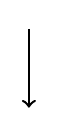
\begin{tikzpicture}\draw[->,line width=0.9pt] (-3,-3) to (-3,-4);\end{tikzpicture}}\overset{\overset{d}{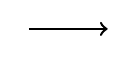
\begin{tikzpicture}\draw[->,line width=0.9pt] (-7,0) to (-6,0);\end{tikzpicture}}}{\left[\begin{array}{ccc}\text{\textemdash} & x_1^\top & \text{\textemdash} \\\text{\textemdash} & x_2^\top & \text{\textemdash} \\ & \vdots &  \\\text{\textemdash} & x_n^\top & \text{\textemdash}\end{array}\right]}=\left[\begin{array}{cccc}| & | &   & | \\x^1 & x^2 & \cdots & x^d \\| & | &   & |\end{array}\right]$$\caption{Dimensions, column and row vector notation for matrix $\mathbf{X}$}\end{figure}
\noindent Let us actually build on the example mentioned above and view the measurements $({x_i})_{j}$ of each sample $\mathbf{x}_i$ as a sequence of measurements, e.g. velocities of car $i$, over time $j = 1,\dots, d$.
\begin{enumerate}
\item Is this problem in a supervised or unsupervised learning setting? \textbf{Please explain.}
\BeginSolution
%5a 
\EndSolution
\item Suppose that we want to learn (from our training set) to predict the location $y$ from only the first $t$ measurements. Denoting the prediction of $y$ at time $t$ by $\hat{y}^t$, we thus want to use $({x})_{j}, j=1, \ldots, t$ to predict $y$. If we now learn how to obtain $\hat{y}^t$ for each $t= 1,\dots,d$, we end up with a sequence of estimators $\hat{y}^1,\dots, \hat{y}^d$ for each car.
\vspace{3pt}

\noindent \textbf{Provide a method to obtain $\hat{y}^t$ for each $t$.} Note that we will obtain a different model for each $t$. 
\BeginSolution
%5b

\EndSolution
\item Someone suggests that maybe the measurements themselves are partially predictable from the previous measurements, which suggests employing a two stage strategy to solve the original prediction problem: First we predict the $t$-th measurement $({x})_{t}$ based on the previous measurements $({x})_{1},\ldots, ({x})_{t-1}$. Then we look at the differences (sometimes deemed the ``innovation'') between the actual $t$-th measurement we obtained and our prediction for it, i.e. $(\Delta \mathbf{x})_{t} := (\mathbf{x})_{t} - (\hat{\mathbf{x}})_{t}$. Finally, we use $(\Delta\mathbf{x})_1,\ldots, (\Delta \mathbf{x})_{t}$ to obtain a prediction $\tilde{y}^t$.
\vspace{3pt}

In order to learn the maps which allow us to (1) take $({x})_{1},\ldots, ({x})_{t-1}$ to obtain $(\Delta\mathbf{x})_1,\ldots, (\Delta \mathbf{x})_{t}$ and (2) take $(\Delta\mathbf{x})_1,\dots, (\Delta \mathbf{x})_{t}$ to predict $\tilde{y}^t$, we again use our training set.  Specifically for each $t$, in stage (1), we fit the vectors of training measurements $\mathbf{x}^1, \ldots, \mathbf{x}^{t-1}$ linearly to $\mathbf{x}^t$ using least squares for each $t$. In stage (2), we use the innovation vectors $(\Delta\mathbf{x}^1, \dots, \Delta\mathbf{x}^t)$ to predict $\mathbf{y}^t$ again using least squares.  Let's define the matrix $\tilde{\mathbf{X}}^t := (\Delta\mathbf{x}^1, \ldots, \Delta\mathbf{x}^t)$ and $\tilde{\mathbf{X}} = \tilde{\mathbf{X}}^d$.
\vspace{3pt}

\textbf{Show how} we can learn the best linear predictions $\hat{\mathbf{x}}^t$ from $\mathbf{x}^1,\ldots, \mathbf{x}^{t-1}$. Then \textbf{provide an expression} for $\tilde{\mathbf{y}}^t$ depending on the innovations $\Delta\mathbf{x}^1,\dots, \Delta\mathbf{x}^{t}$.
\vspace{3pt}

When presented with a new feature vector $\mathbf{x}$, are the sequence of final predictions of the one-stage training $\hat{y}^t$ in (a) and two-stage training $\tilde{y}^t$ in (b) the same?  \textbf{Explain your reasoning.}
\BeginSolution
%5c

\EndSolution
\item \textbf{Which well-known procedure do the steps to obtain $\tilde{\mathbf{X}}$ from $\mathbf{X}$ remind you of}? (\textbf{HINT: } Think about how the column vectors in $\tilde{\mathbf{X}}$ are geometrically related.)

\textbf{Is there an efficient way to update the weight vector $\hat{\mathbf{w}}^{t}$ from $\hat{\mathbf{w}}^{t-1}$ when computing the sequence of predictions $\tilde{y}^t$?}
\BeginSolution
%5d

\EndSolution
\item Now let's consider the more general setting where we now want to predict a target vector $\mathbf{y} \in \mathbb{R}^k$ from a feature vector $\mathbf{x} \in \mathbb{R}^d$, thus having a training set consisting of observations $(\mathbf{x}_i, \mathbf{y}_i)$ for $i=1,\ldots,n$.
\vspace{3pt}

Instead of learning a weight vector $\mathbf{w} \in \mathbb{R}^d$, we now want a linear estimate $\hat{\mathbf{y}} = \hat{\mathbf{W}} \mathbf{x}$ with a weight matrix $\hat{\mathbf{W}} \in \mathbb{R}^{k\times d}$ instead. From our samples, we obtain wide matrices $\mathbf{Y} \in \mathbb{R}^{k\times n}$ with columns $\mathbf{y}_1,\ldots,\mathbf{y}_n$ and $\mathbf{X} \in \mathbb{R}^{d\times n}$ with columns $\mathbf{x}_1, \ldots,\mathbf{x}_n$ (note that this is the transpose of $\mathbf{X}$ in Figure 2). In order to learn $\hat{\mathbf{W}}$ we now want to minimize $\|\mathbf{Y} - \mathbf{W}\mathbf{X}\|_F^2$ where $\|\cdot\|_F$ denotes the Frobenius norm of matrices, i.e. $\|\mathbf{L}\|_F^2 = \operatorname{trace}(\mathbf{L}^\top\mathbf{L})$.
\vspace{3pt}

\textbf{Show how to find $\hat{\mathbf{W}} = \arg\min_{\mathbf{W} \in \mathbb{R}^{d\times d}} \|\mathbf{Y} - \mathbf{W}\mathbf{X}\|_F^2$ using vector calculus as reviewed in Discussion 0 and 1.}
\BeginSolution
%5e

\EndSolution
\item In the setting of problem (e), \textbf{argue why} the computation of the best linear prediction $\hat{\mathbf{y}}$ of a target vector $\mathbf{y}$ using a feature vector $\mathbf{x}$ can be solved by separately finding the best linear prediction for each measurement $({y})_{j}$ of the target vector $\mathbf{y}$.
\BeginSolution
%5f

\EndSolution
\end{enumerate}
%%%% Problem 5 Ends Here %%%%
\clearpage

%%%% Problem 6 Starts Here %%%%
\vspace{-2mm}\noindent\begin{mybox}{\begin{center}\textbf{\color{black}Problem 6: System Identification by Ordinary Least Squares Regression}\end{center}}\end{mybox}\vspace{-2mm}
\vspace{10pt}
\noindent Making autonomous vehicles involves machine learning for different purposes. One of which is learning how cars actually behave based on their data.
\vspace{3pt}

\noindent \textbf{Make sure to submit the code you write in this problem to ``HW1 Code'' on Gradescope.}
\begin{enumerate}
\item Consider the time sequence of scalars $x_t \in \mathbb{R}$ and $u_t \in \mathbb{R}$ in which $x_{t+1} \approx A  x_{t} + B u_{t}$.  In control theory, $x_t$ usually represents the state, and $u_t$ usually represents the control input.  \textbf{Find the numbers $A$ and $B$ so that $\sum_t(x_{t+1} - A  x_{t} - B u_{t})^2$ is minimized.} The values of $x_t$ and $u_t$ are stored in \texttt{a.mat}.
\BeginSolution
%6a

\EndSolution
\item Consider the time sequences of vectors $\mathbf{x}_t \in \mathbb{R}^3$ and $\mathbf{u}_t \in \mathbb{R}^3$ in which $\mathbf{x}_{t+1} \approx \mathbf{A} \mathbf{x}_{t} + \mathbf{B} \mathbf{u}_{t}$. \textbf{Find the matrix $\mathbf{A} \in \mathbb{R}^{3\times 3}$ and $\mathbf{B} \in \mathbb{R}^{3\times 3}$ so that the sum of the squared $\ell^2$-norms of the error, $\sum_t\|\mathbf{x}_{t+1} - \mathbf{A} \mathbf{x}_{t} - \mathbf{B} \mathbf{u}_{t}\|_2^2$, is minimized}.  The values of $\mathbf{x}_t$ and $\mathbf{u}_t$ are stored in \texttt{b.mat}.
\BeginSolution
%6b

\EndSolution
\item Consider a \textit{car following model} that models how cars line up on a straight $1$-d highway at a given time.  The acceleration of a car can be approximated by a linear function of the positions and velocities of its own and the car in front of it.  Mathematically, we can formulate this as $$\ddot{x}_i \approx a x_{i} + b \dot{x}_{i} + c x_{i-1} + d \dot{x}_{i-1} + e,$$ where $x_i$, $\dot x_i$, and $\ddot x_i$ are the position, velocity, and acceleration of the $i$th car in the line.
\vspace{3pt}

\textbf{Find $a$, $b$, $c$, $d$, and $e$ that minimizes $$\sum_i \| -\ddot{x}_i + a x_{i} + b \dot{x}_{i} + c x_{i-1} + d \dot{x}_{i-1} + e\|_2^2$$ using data file \texttt{train.mat}}, which contains the status of 40\,000 cars at a given point from the I-80 highway in California. The data were sampled from the Next Generation Simulation (NGSIM) dataset so that the $i$ may not be continuous.  For your convenience, we give you the profiles of each sampled car and the car that is in front of it.
\BeginSolution
%6c

\EndSolution
\item \textbf{Try to justify why your result in (c) is physically reasonable.}  Hint: You can reorganize your equation to be $$\ddot{x}_i = h (x_{i-1}- x_{i}) + f (\dot{x}_{i-1} - \dot{x}_{i}) - g (\dot{x}_{i}-L)+ w_i,$$ and try to explain the physical meaning for each term, with $L$ being the speed limit.
\BeginSolution
%6d

\EndSolution
\end{enumerate}
%%%% Problem 6 Ends Here %%%%
\clearpage

%%%% Problem 7 Starts Here %%%%
\vspace{-2mm}\noindent\begin{mybox}{\begin{center}\textbf{\color{black}Problem 7: A Simple Classification Approach}\end{center}}\end{mybox}\vspace{-2mm}
\vspace{10pt}
\noindent \textbf{Make sure to submit the code you write in this problem to ``HW1 Code'' on Gradescope.}
\vspace{3pt}

\noindent Classification is an important problem in applied machine learning and is used in many different applications like image classification, object detection, speech recognition, machine translation and others.
\vspace{3pt}

\noindent In \textit{classification}, we assign each datapoint a class from a finite set (for example the image of a digit could be assigned the value $0, 1, \ldots, 9$ of that digit). This is different from \textit{regression}, where each datapoint is assigned a value from a continuous domain like $\mathbb{R}$ (for example features of a house like location, number of bedrooms, age of the house, etc. could be assigned the price of the house).
\vspace{3pt}

\noindent In this problem we consider the simplified setting of classification where we want to classify data points from $\mathbb{R}^d$ into \textit{two} classes. For a linear classifier, the space $\mathbb{R}^d$ is split into two parts by a hyperplane: All points on one side of the hyperplane are classified as one class and all points on the other side of the hyperplane are classified as the other class.
\vspace{3pt}

\noindent The goal of this problem is to show that even a regression technique like linear regression can be used to solve a classification problem. This can be achieved by regressing the data points in the training set against $-1$ or $1$ depending on their class and then using the level set of 0 of the regression function as the classification hyperplane (i.e. we use 0 as a threshold on the output to decide between the classes).
\vspace{3pt}

\noindent Later in lecture we will learn why linear regression is not the optimal approach for classification and we will study better approaches like logistic regression, SVMs and neural networks.
\begin{enumerate}
\item The dataset used in this exercise is a subset of the MNIST dataset. The MNIST dataset assigns each image of a handwritten digit their value from $0$ to $9$ as a class. For this problem we only keep digits that are assigned a $0$ or $1$, so we simplify the problem to a two-class classification problem.
\vspace{3pt}

\textbf{Download and visualize the dataset (example code included). Include three images that are labeled as $0$ and three images that are labeled as $1$ in your submission.}
\BeginSolution
%7a

\EndSolution
\item We now want to use linear regression for the problem, treating class labels as real values $y = -1$ for class ``zero'' and $y = 1$ for class ``one''. In the dataset we provide, the images have already been flattened into one dimensional vectors (by concatenating all pixel values of the two dimensional image into a vector) and stacked as rows into a feature matrix $\mathbf{X}$. We want to set up the regression problem $\min_{\mathbf{w}}\norm{\mathbf{X}\mathbf{w} - \mathbf{y}}_2^2$ where the entry $y_i$ is the value of the class ($-1$ or $1$) corresponding to the image in row $\mathbf{x}_i^\top$ of the feature matrix. \textbf{Solve this regression problem for the training set and report the value of $\|\mathbf{X}\mathbf{w} - \mathbf{y}\|_2^2$ as well as the weights $\mathbf{w}$.} For this problem you may only use pure Python and NumPy (no machine learning libraries!).
\BeginSolution
%7b

\EndSolution
\item Given a new flattened image $\mathbf{x}$, one natural rule to classify it is the following one: It is a zero if $\mathbf{x}^\top \mathbf{w} \leqslant 0$ and a one if $\mathbf{x}^\top \mathbf{w} > 0$. \textbf{Report what percentage of the digits in the training set are correctly classified by this rule. Report what percentage of the digits in the test set are correctly classified by this rule.}
\BeginSolution
%7c

\EndSolution
\item \textbf{Why is the performance typically evaluated on a separate test set (instead of the training set) and why is the performance on the training and test set similar in our case?} We will cover these questions in more detail later in the class.
\BeginSolution
%7d

\EndSolution
\item Somebody suggests to use 0 (for class 0) and 1 (for class 1) as the entries for the target vector $\mathbf{b}$. Try out how well this is doing (make sure to adapt the classification rule, i.e. the threshold set for the outputs). \textbf{Report what percentage of digits are correctly classified using this approach on the training set and test set.} How are the performances of the two approaches if you add a bias column to the feature matrix $\mathbf{X}$? A bias column is a column of all ones, i.e. the new feature matrix $\mathbf{X}'$ is $$\mathbf{X}' = \begin{bmatrix}\mathbf{x}_0^\top & 1\\\mathbf{x}_1^\top & 1\\ \vdots & \vdots \\ \mathbf{x}_n^\top & 1 \end{bmatrix}$$ \textbf{Report what percentage of digits are correctly classified using regression targets $0/1$ and $-1/1$ with bias on the training set and test set.} \textbf{Try to explain the results!}
\BeginSolution
%7e

\EndSolution
\end{enumerate}
%%%% Problem 7 Ends Here %%%%
\clearpage

%%%% Problem 8 Starts Here %%%%
\vspace{-2mm}\noindent\begin{mybox}{\begin{center}\textbf{\color{black}Problem 8: Your Own Question}\end{center}}\end{mybox}\vspace{-2mm}
\vspace{10pt}
\noindent \textbf{Write your own question, and provide a thorough solution.}
\vspace{3pt}

\noindent Writing your own problems is a very important way to really learn the material. The famous ``Bloom's Taxonomy'' that lists the levels of learning is: Remember, Understand, Apply, Analyze, Evaluate, and Create. Using what you know to create is the top-level. We rarely ask you any HW questions about the lowest level of straight-up remembering, expecting you to be able to do that yourself. (e.g. make yourself flashcards) But we don't want the same to be true about the highest level.
\vspace{3pt}

\noindent As a practical matter, having some practice at trying to create problems helps you study for exams much better than simply counting on solving existing practice problems. This is because thinking about how to create an interesting problem forces you to really look at the material from the perspective of those who are going to create the exams. 
\vspace{3pt}

\noindent Besides, this is fun. If you want to make a boring problem, go ahead. That is your prerogative. But it is more fun to really engage with the material, discover something interesting, and then come up with a problem that walks others down a journey that lets them share your discovery. You don't have to achieve this every week. But unless you try every week, it probably won't happen ever. 
\BeginSolution
\EndSolution
%%%% Problem 8 Ends Here %%%%
\clearpage

\end{document}
%%%%% Template Ends Here %%%%%